\section{Proposed Verification Tool Flow}
%
\begin{figure}[t]
\centering
\vspace*{0.3cm}
\scalebox{.55}{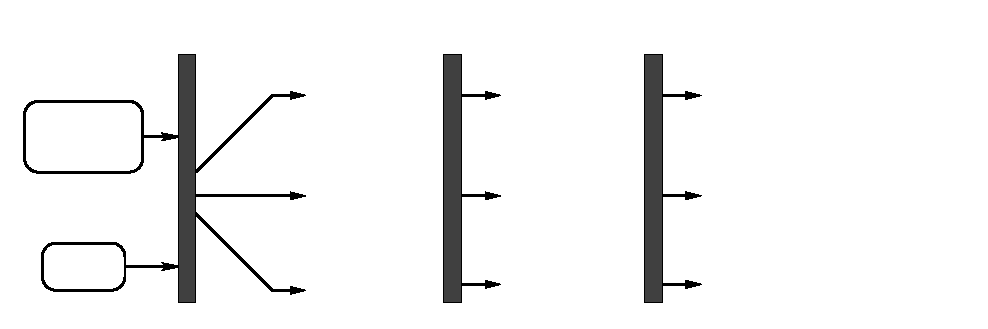
\includegraphics{figures/new_flow_pspdftex.eps}}
\caption{Tool flow for hardware property verification\label{fig:toolflow}}
\end{figure}
%
%===============================================================================
%\subsection{Software Verifiers at the heart of Hardware Verification}
%===============================================================================
%
Figure~\ref{fig:toolflow} gives the tool flow for hardware RTL 
verification using bit-level netlist, word-level netlist and software netlist.  
The bottom flow of Figure~\ref{fig:toolflow} shows the bit-level 
verification flow using ABC.
ABC does not support Verilog, so we use an open-source synthesis tool,
\yosys\footnote{http://www.clifford.at/yosys/} to translate Verilog
RTL to BLIF or AIGER~\footnote{http://fmv.jku.at/aiger/FORMAT-20070427.pdf} 
which is then passed to ABC for verification. 
%Given a design in Verilog RTL, \yosys bit-blasts it into a bit-level netlist 
%along with the property and the resultant netlist is expressed in AIG.  
%The AIG is represented in AIGER format  which is one of the standards 
%andmost prevalant format used by the majority of verification tools.
Whereas, the middle flow of Figure~\ref{fig:toolflow} shows the 
bit/word-level verification using the tool 
\ebmc~\footnote{www.cprover.org/hardware/ebmc}. 
\ebmc supports IEEE 1364.1 Verilog 2005 standards.  \ebmc synthesize 
the design in Verilog into a bit-level netlist represented in AIGER or a 
word-level netlist represented in format that resembles the 
SMT-LIB standard. The word-level synthesis flow in \ebmc is not mature yet. 
So, we only use the bit-level flow in \ebmc. 
%
The top flow of Figure~\ref{fig:toolflow} shows the verification 
of the software netlist designs. 
%verification which translate RTL into software netlist using the tool \emph{v2c}.  
%
A wide range of representative software 
verification techniques is applied to determine the safety of the
software netlist. In particular, we use $k$-induction~\cite{fmcad2000}
(implemented in the tools CBMC~\cite{cbmc.tacas:2004} and
2LS~\cite{BJKS15}), interpolation
(CPAChecker~\cite{DBLP:conf/cav/BeyerK11}, IMPARA~\cite{impara}), 
Abstract Interpretation (Ast{\'r}ee~\cite{DBLP:conf/esop/CousotCFMMMR05}), 
IC3/PDR (SeaHorn~\cite{DBLP:conf/cav/GurfinkelKKN15}) and Automata-theoretic 
verification (UltimateAutomizer~\cite{DBLP:conf/tacas/HeizmannDGLMSP16}).
%
%===============================================================================
\section{Experimental Results}\label{sec:results}
%===============================================================================
In this section, we report experimental results for \emph{unbounded} safety 
verification of hardware RTL.  Our experimental contributions are two folds.
%
\begin{enumerate}
  \item Compare off-the-shelf formal verification tools for RTL designs by translating  
     them to \emph{bit-level netlist} and \emph{software netlist}.  
    To this end, we compare state-of-the-art hardware model checking tools, such as 
    \emph{ABC 1.01} (winner of HWMCC'15) and 
    \ebmcv~\footnote{\scriptsize{www.cprover.org/hardware/ebmc}}, 
    with various software analyzers from SV-COMP 2016, such as 
    \emph{UltimateAutomizer 3292eade} (winner of SV-COMP'16), 
    \emph{CPAChecker 1.4}, 
    \emph{SeaHorn (revision 07666c810d)}, \emph{2LS 0.3.4}, 
    and a commercial abstract 
    interpretation based tool, \emph{Astr{\'e}e}.  
  
 \item  Compare the performance of unbounded verification algorithms such as $k$-induction, 
    Interpolation, IC3/PDR and Abstraction Interpretation for generating proofs as well as 
    finding complex bugs. 
\end{enumerate}
%
Our experiments were performed on an Intel Xeon machine running at
3.07\,GHz.  We restricted the resources to 5 hours and 32\,GB RAM per
benchmark.  All our benchmarks in Verilog, software netlist in C, 
scripts for running \yosys, ABC, \ebmcv, and other software 
verification tools are available here.~\footnote{\scriptsize{https://github.com/rajdeep87/TCAD-experiments}}
%to a publicly accessible archive website.
%\footnote{\scriptsize{http://www.cprover.org/hardware/tcad/}}
%
%===============================================================================
\subsection{Benchmarks}
%===============================================================================
%
We verified a total of~34 circuits given in Verilog RTL.  Out of 34, 26 
are \emph{safe} benchmarks and 8 are \emph{unsafe}.  The benchmarks in 
our paper are derived from real world hardware benchmark suites, including 
VIS Verilog models, the Texas-97 Benchmark suite, and opencores.org. We synthesize 
each benchmarks into three different netlist formats -- AIGER, SMT-LIB2, ANSI-C.
We classify our benchmarks into two different classes -- data-path intensive
circuits, including Huffman encoder/decoder and a Digital Audio
Input-Output chip (DAIO); and control-intensive designs,
including a non-pipelined 3-stage processor, a Read-Copy-update
mutual exclusion protocol, a FIFO controller, a buffer allocation model,
and an instruction queue controller.   
%
%-------------------------------------------------------------------------------
\subsection{Properties}
%-------------------------------------------------------------------------------
%
The safety properties are specified as System Verilog Assertions.
The SVA properties are translated into C assertions and instrumented 
in the software netlist. 
%
Below, we present few examples of the concurrent assertions in SVA 
and corresponding assertions in the software netlist design.  


Figure~\ref{figure:prop1} and Figure~\ref{figure:prop2} gives 
the SVA property on the left and the corresponding assertions 
in software netlist on the right for the vending machine benchmark 
and Huffman encoder/decoder benchmark, respectively. For the purpose 
of illustration we give partial code fragments for the software 
netlist designs.
%
\begin{example}~\label{safety-prop}
$Assert\_1$: {\em The balance is never negative and never reaches 15.} 
%\vspace{-3mm}
\begin{figure}[htbp]
\centering
\scriptsize
\begin{tabular}{l|l}
\hline
SVA & Assertion (in C)
\\
\hline
\begin{lstlisting}[mathescape=true,language=Verilog]
p1: assert property 
 (@(posedge clk) 
 vending.total[3]==0 && 
 !(vending.total[4:0]==15)); 
\end{lstlisting}
&
\begin{lstlisting}[mathescape=true,language=C]
 assert((((vending.total 
 >> 3) & 0x1) == 0) 
 && !(vending.total 
 & 0x1F == 15));
\end{lstlisting} \\
\hline
\end{tabular}
\caption{Modeling concurrent SVA in software netlist}
\label{figure:prop1}
\end{figure}
%
\end{example}
%
\begin{example}~\label{safety-propnew}
$Assert\_2$: {\em When a new transmission begins, the decoder is ready in the next clock.}
%
\begin{figure}[htbp]
\centering
\scriptsize
\begin{tabular}{l|l}
\hline
SVA & Assertion (in C)
\\
\hline
\begin{lstlisting}[mathescape=true,language=Verilog]
p2: assert property 
 (@(posedge clk) 
 encoder.shiftreg[9:1] 
 == 1 |-> ##1 
 decoder.leaf == 1);
\end{lstlisting}
&
\begin{lstlisting}[mathescape=true,language=C]
 if(((encoder.shiftreg >> 1) 
 & 0x1FF) == 1) {
  // call to top level 
  // module of design
  huffman(clk,addr);  
  assert(decoder.leaf == 1);
 }
\end{lstlisting} \\
\hline
\end{tabular}
\caption{Modeling temporal properties in SVA in software netlist}
\label{figure:prop2}
\end{figure}
\end{example}

%
%-------------------------------------------------------------------------------
\subsection{Discussion}
%-------------------------------------------------------------------------------
We classify the analysis results into two categories -- 1) \emph{precise} tools 
that do not use any abstraction and performs precise reasoning using SAT/SMT solvers 
(in section~\ref{precise}), and \emph{abstraction} based tools that performs 
approximate analysis without using SAT/SMT solvers (in section~\ref{abstraction}). 
%
\subsection{Analysis Using Precise tools}~\label{precise}
%
Figures~\ref{fig:kind}--\ref{fig:hybrid} report the comparison of various unbounded 
verification techniques employed by verification tools at bit-level, word-level, 
and software-level.  The plots in these figures reports the runtimes of~12 
representative circuits which are most difficult to solve out of a total~34 
circuits.  Note that ABC does not implement word-level verification flow, 
so we perform word-level verification using our in-house tool \ebmc.
Figures~\ref{fig:kind}--\ref{fig:hybrid} reports the best runtimes 
among the bit-level and word-level hardware verification tools.  
%
We categorize the unbounded approaches into three classes:
\begin{itemize}
\item $k$-induction (Figure~\ref{fig:kind})
\item interpolation (Figure~\ref{fig:impact}), and 
\item PDR together with other hybrid techniques (Figure~\ref{fig:hybrid}).  
\end{itemize}
By hybrid techniques, we refer to predicate
abstraction as implemented in \emph{CPAChecker} and a combination of
$k$-induction, BMC and abstract interpretation as implemented in
\emph{2LS}~\cite{kiki}.  On the $x$-axis is the analysis time in
seconds and on the $y$-axis we list the benchmarks. The vertical red lines on
the right-hand side of the diagrams show timeouts, out of memory,
inconclusive (unknown) results, errors (crashes), and wrong results
(tool bugs) reported by the tools. The tools can be distinguished 
by the size of the circles as well as by colour. 

\subsection{Analysis using $k$-induction} For safe benchmarks, the results
for bit-level, word-level verifiers and software verifiers are
comparable when the properties are 1-inductive or 2-step inductive.
However, for complex safety properties, ABC and other abstraction
based software analyzers either timeout or took a long time to
terminate.  We investigated the reason for higher verification times
for some safe benchmarks, such as the FIFO controller, the RCU, and Buffer 
Allocation.  We observe that the properties are not $k$-inductive for
sufficiently large values of $k$, e.g.\ (k=1000) and thus tools based
on $k$-induction either timeout or took long time to
compute the inductive invariant sufficient to prove the property. For
the unsafe benchmarks, for example DAIO and the traffic light controller, where
the bugs are manifested only at 64 and 65 clock cycles respectively,
the verification times using ABC and \ebmc's $k$-induction engine 
are comparable to \cbmcv and \textsc{2LS}. Figure~\ref{fig:kind} 
reports the time taken by the $k$-induction engine in 
ABC, \ebmcv, \cbmcv and \textsc{2LS}.  We did not report
the time for \emph{CPAChecker} since the results suggest that 
its $k$-induction engine is not as mature yet. 

\subsection{Analysis using Interpolation} Figure~\ref{fig:impact} reports
the time taken by the interpolation engine in ABC, \textsc{IMPARA}
and \emph{CPAChecker}. ABC is the fastest in 9 out of 12
designs. However, it timed out on three complex benchmarks, RCU, FIFO
and BufAl, whereas the software interpolation tool, \textsc{IMPARA},
which implements IMPACT algorithm solved three instances out of which
one is the complex FIFO design; yet \textsc{IMPARA} either timed out or
ran out of memory for the remaining designs.  \emph{CPAChecker} solved
5 out of 12 cases.  None of the interpolation engines was able to
prove RCU and BufAl.

\subsection{Analysis using Hybrid techniques} Figure~\ref{fig:hybrid}
reports the time taken by the IC3/PDR engine in ABC, \emph{SeaHorn}
and other hybrid techniques as implemented in \emph{CPAChecker} and
\textsc{2LS}. ABC~is the clear winner here; it is the only tool that
proves the FIFO and BufAl benchmarks safe within the given 5h timeout.
\emph{SeaHorn}'s PDR engine solves half of the benchmarks, but
produces false negatives on the other half due to limited support for
bitvectors. \textsc{2LS} successfully solved 8 benchmarks and times 
out on four benchmarks.  \emph{CPAChecker}'s predicate abstraction reliably
solves 7 benchmarks, but timed out on two benchmarks and reports three
wrong results. Note that none of the tools was able to prove RCU.

\Omit{
The bit-level hardware tools performs better than word-level hardware 
verification for our benchmarks.  So, we only report the bit-level results 
obtained using ABC in Figures~\ref{fig:kind}--\ref{fig:hybrid}.
}


%We do not report the results using Astr{\'e}e since it requires manual
%directives for data and control partitioning to avoid imprecision;
%nonetheless it generates many false alarms for safe benchmarks.

%
%%%%%%%%%%%%%%%%%%%%%%%%%%%%%%%%%%%%%%%%%%%%%%%%%%%%%%%%%%%%%%%%%%%%%%%%%%%%%%%%
\begin{figure}
%\scalebox{0.9}{
\begin{tikzpicture}[scale=0.9]
\small
\pgfplotstableread{
Benchmark	ABC-kind	EBMC-kind	CBMC-kind	2LS-kind
BufAl	15000	15000	15000	15000
DAIO	59.92	73.62	229.72	54
Dekker	0.17	15000	15000	15000
FIFOs	15000	15000	15000	15000
Heap	0.34	15000	15000	15000
Huffman	0.02	0.01	0.21	0.24
Ibuf	0.01	0.01	0.26	0.3
RCU	15000	15000	15000	15000
TicTacToe	0.01	0.01	0.23	0.25
n-pipe-mp	0.02	0.26	0.27	0.17
traffic-light	1.52	32.67	29.46	7.98
Vending	0.02	0.02	0.21	0.25
}\datatable

\begin{axis}[
    xbar, xmode=log,
    xmin=0,         
    ytick=data,    
    yticklabels from table={\datatable}{Benchmark},  
    legend style={at={(0.9,1.3)}},
]
\addplot [mark size=5pt,only marks, fill=yellow] table [x={ABC-kind}, y expr=\coordindex] {\datatable};    
\addplot [mark size=4pt,only marks, fill=green!70!blue]table [x={EBMC-kind}, y expr=\coordindex] {\datatable};
\addplot [mark size=3pt,only marks, fill=red!80!yellow] table [x={CBMC-kind}, y expr=\coordindex] {\datatable};
\addplot [mark size=2pt,only marks, fill=blue] table [x={2LS-kind}, y expr=\coordindex] {\datatable};
\addplot [red,sharp plot] coordinates{(15000,0) (15000,11)}
          node [left,rotate=90] at (axis cs:9000,10) {timeout};
\legend{{ABC-kind},{EBMC-kind},{CBMC-kind},{2LS-kind}}
\end{axis}
\end{tikzpicture}
%}
\caption{\label{fig:kind}
Comparison of $k$-induction tools
}
\end{figure}
%%%%%%%%%%%%%%%%%%%%%%%%%%%%%%%%%%%%%%%%%%%%%%%%%%%%%%%%%%%%%%%%%%%%%%%%%%%%%%%%

%%%%%%%%%%%%%%%%%%%%%%%%%%%%%%%%%%%%%%%%%%%%%%%%%%%%%%%%%%%%%%%%%%%%%%%%%%%%%%%%
\begin{figure}
%\scalebox{0.9}{
\begin{tikzpicture}[scale=0.9]
\small
\pgfplotstableread{
Benchmark	ABC-interpolation	CPA-interpolation	IMPARA-interpolation
BufAl	15000	60000	15000
DAIO	65.74	60000	240000
Dekker	3.73	240000	30000
FIFOs	15000	240000	0.39
Heap	1215.79	60000	15000
Huffman	0.01	3.87	0.41
Ibuf	0.01	4.04	30000
RCU	15000	60000	15000
TicTacToe	0.04	3.3	7870
non-pipe-mp	0.01	3.44	120000
traffic-light	5.79	240000	15000
Vending	0.01	3.65	120000
}\datatable

\begin{axis}[
    xbar, xmode=log,
    xmin=0,         
    ytick=data,    
    yticklabels from table={\datatable}{Benchmark},  
    legend style={at={(0.9,1.2)}},
]
\addplot [mark size=4pt,only marks, fill=yellow] table [x={ABC-interpolation}, y expr=\coordindex] {\datatable};    
\addplot [mark size=3pt,only marks, fill=orange]table [x={CPA-interpolation}, y expr=\coordindex] {\datatable};
\addplot [mark size=2pt,only marks, fill=gray] table [x={IMPARA-interpolation}, y expr=\coordindex] {\datatable};
\addplot [red,sharp plot] coordinates{(15000,0) (15000,11)}
          node [left,rotate=90] at (axis cs:9000,11) {timeout};
\addplot [red,sharp plot] coordinates{(30000,0) (30000,11)}
          node [left,rotate=90] at (axis cs:19000,11) {memout};
\addplot [red,sharp plot] coordinates{(60000,0) (60000,11)}
          node [left,rotate=90] at (axis cs:40000,11) {unknown};
\addplot [red,sharp plot] coordinates{(120000,0) (120000,11)}
          node [left,rotate=90] at (axis cs:80000,11) {error};
\addplot [red,sharp plot] coordinates{(240000,0) (240000,11)}
          node [left,rotate=90] at (axis cs:180000,11) {wrong};
\legend{{ABC-interpolation},{CPA-interpolation},{IMPARA}}
\end{axis}
\end{tikzpicture}
%}
\caption{\label{fig:impact}
Comparison of interpolation-based tools
}
\end{figure}
%%%%%%%%%%%%%%%%%%%%%%%%%%%%%%%%%%%%%%%%%%%%%%%%%%%%%%%%%%%%%%%%%%%%%%%%%%%%%%%%

%%%%%%%%%%%%%%%%%%%%%%%%%%%%%%%%%%%%%%%%%%%%%%%%%%%%%%%%%%%%%%%%%%%%%%%%%%%%%%%%
\begin{figure}
%\scalebox{0.9}{
\begin{tikzpicture}[scale=0.9]
\small
\pgfplotstableread{
Benchmark	ABC-pdr	SeaHorn-pdr	CPA-predabs	2LS-kiki
BufAl	12250.5	240000	240000	15000
DAIO	0.03	2.16	3.95	55.72
Dekker	0.03	4.83	240000	15000
FIFOs	3759.75	240000	15000	15000
Heap	0.75	240000	10.09	0.91
Huffman	0.02	0.09	4.01	0.25
Ibuf	0.01	240000	3.95	0.73
RCU	15000	240000	15000	15000
TicTacToe	0.03	240000	3.29	0.21
non-pipe-mp	0.01	0.06	3.46	0.20
traffic-light	0.13	1.44	240000	7.48
Vending	0.02	1.28	3.77	0.34
}\datatable

\begin{axis}[
    xbar, xmode=log,
    xmin=0,         
    ytick=data,    
    yticklabels from table={\datatable}{Benchmark},  
    legend style={at={(0.9,1.3)}},
]
\addplot [mark size=5pt,only marks, fill=yellow] table [x={ABC-pdr}, y expr=\coordindex] {\datatable};    
\addplot [mark size=4pt,only marks, fill=green!70!blue]table [x={SeaHorn-pdr}, y expr=\coordindex] {\datatable};
\addplot [mark size=3pt,only marks, fill=orange] table [x={CPA-predabs}, y expr=\coordindex] {\datatable};
\addplot [mark size=2pt,only marks, fill=blue] table [x={2LS-kiki}, y expr=\coordindex] {\datatable};
\addplot [red,sharp plot] coordinates{(15000,0) (15000,11)}
          node [left,rotate=90] at (axis cs:9000,11) {timeout};
\addplot [red,sharp plot] coordinates{(30000,0) (30000,11)}
          node [left,rotate=90] at (axis cs:19000,11) {memout};
\addplot [red,sharp plot] coordinates{(60000,0) (60000,11)}
          node [left,rotate=90] at (axis cs:40000,11) {unknown};
\addplot [red,sharp plot] coordinates{(120000,0) (120000,11)}
          node [left,rotate=90] at (axis cs:80000,11) {error};
\addplot [red,sharp plot] coordinates{(240000,0) (240000,11)}
          node [left,rotate=90] at (axis cs:180000,11) {wrong};
\legend{{ABC-pdr},{SeaHorn-pdr},{CPA-predabs},{2LS-kiki}}
\end{axis}
\end{tikzpicture}
%}
\caption{\label{fig:hybrid}
Comparison of hybrid techniques
}
\end{figure}
%
%%%%%%%%%%%%%%%%%%% Plot runtimes %%%%%%%%%%%%%%%%%%%%%%%
\begin{figure}[t]
  \centering
  \begin{tikzpicture}[scale=0.60]

\pgfplotscreateplotcyclelist{markstyles}{%
solid, every mark/.append style={solid, fill=white}, mark=square*, mark size=2.5\\%
solid, every mark/.append style={solid, blue}, mark=triangle*,mark size=2.5\\%
solid, every mark/.append style={solid, fill=black}, mark=otimes*,, mark
    size=2.5\\%
}
    
 	%axis
  \begin{axis}[
    width=\linewidth,
    xlabel={Benchmark Number},
    ylabel={Time (seconds)},
    domain = 1:40,
    xmin=1, xmax=34,
    ymin=0, ymax=200,
    %ytick={0,20,...,200},
    xtick={1,5,10,...,34},
    width=15cm, height= 7cm,
    ymode = log,
    %log basis x={2},
    %xticklabel=\pgfmathparse{2^\tick}\pgfmathprintnumber{\pgfmathresult},
    legend pos = north west,
    grid = major,
    major grid style={line width=.2pt,draw=gray!50},
    cycle list name=markstyles
  ]
	
  %plots
  %\addplot table [only marks, y=Time, x=Benchmarks]{plotdata/cbmc.dat};
	%\addlegendentry{CBMC}
  
  \addplot table [only marks, y=Time, x=Benchmark]{plotdata/ultimate.dat};
  \addlegendentry{UltimateAutomizer}
  
  \addplot table [only marks, y=Time, x=Benchmark]{plotdata/astree.dat};
  \addlegendentry{Astr{\'e}e}
	
  \end{axis}  
\end{tikzpicture}
\caption{\label{fig:runtimes}
  Runtime Comparison between UltimateAutomizer and Astr{\'e}e}
\end{figure}

%%%%%%%%%%%%%%%%%%%%%%%%%%%%%%%%%%%%%%%%%%%%%%%%%%%%%%%%%

%
%%%%%%%%%%%%%%%%%%%%%%%%%%%%%%%%%%%%%%%%%%%%%%%%%%%%%%%%%%%%%%%%%%%%%%%%%%%%%%%%
\subsection{Bit-level versus Word-level Analysis}
%%%%%%%%%%%%%%%%%%%%%%%%%%%%%%%%%%%%%%%%%%%%%%%%%%%%%%%%%%%%%%%%%%%%%%%%%%%%%%%%
%
Figure~\ref{fig:solverruntimes} gives the runtime comparison between bit-level 
model checking using SAT solvers and word-level model checking using SMT solvers.  
% 
The SAT (in DIMACS format) and SMT (in SMT-LIB2 format) benchmarks are obtained 
automatically using CBMC from the software netlist design. 
%  
For bit-level results, we report the best runtimes among MiniSAT~\cite{minisat} 
and Lingeling~\cite{lingeling} solvers.  The word-level results are obtained 
using Boolector~\cite{boolector} SMT solver which solved more instances 
than Z3~\cite{z32008} SMT solver. 
%  
The timeout was set to~200 seconds per benchmark.  
%
The runtimes in Figure~\ref{fig:solverruntimes} are obtained for 
a pre-determined unwind bound of~70.  The bit-level engine in CBMC 
wins consistently over the word-level engine, except for the 5~cases 
where Boolector was faster than the bit-level solvers.   
% 
We investigate the reason for the higher runtimes of the 
word-level engine. We observe that the RTL designs used 
for our experiment contains too many bit-slices. 
%, which is also exhibited by the software netlist 
%designs due to the bit-precise translation. 
Hence, pure word-level reasoning performs poorly compared 
to the bit-level analysis since word-level tools also use 
bit blasting for solving such designs. 
%
\subsection{Analysis Using Abstraction based tools}~\label{abstraction}
%
One of the benefits of the proposed tool flow in this paper is that the 
synthesis of RTL to software netlist enables the application of techniques 
such as abstract interpretation. Abstract Interpretation~\cite{Cousot92,CC79} 
is a theory of sound approximation of program semantics based on lattice 
structures. Static analysis using abstract interpretation is widely used 
to verify properties of safety-critical systems. 


Astr{\'e}e~\cite{DBLP:conf/esop/CousotCFMMMR05} is a commercial abstract 
interpretation tool developed by AbsInt~\footnote{https://www.absint.com/}.  
It is primarily used for static analysis of safety-critical softwares 
such as avionics software~\cite{DBLP:journals/corr/abs-cs-0701193}.
Astr{\'e}e employs numeric abstract domains, such as intervals that  
abstract variable values as ranges, as well as relational domains that  
infer linear and non-linear relationships between variables. These abstractions are  
well-suited for programs performing integer and float arithmetic, but  
less so for bit-level Boolean operators, bit-shifts, and bitfields  
packing several values in words.  The non-linear abstract domains in 
Astr{\'e}e such as quadratic and exponential functions are mostly useful 
for aerospace applications~\cite{DBLP:journals/ftpl/BertraneCCFMMR15}.  
Moreover, Astr{\'e}e features BDD-based abstract 
domains~\cite{bdd-domain} that can represent non-convex invariants, 
but they are currently limited to Boolean variables and cannot perform  
bit-blasting on integer variables.  For bit manipulating programs 
generated by \textsc{v2c}, Astr{\'e}e uses default abstract domains 
for integer values such as interval domain, octagon domain, integer 
congruences, integer bitfields, and finite sets (of possible values).


When Astr{\'e}e encounters an \texttt{assert}, it first checks whether 
there are some program states that do not satisfy the assertion, and 
then continues the analysis with only the states that satisfy the assertion. 
Indeed, it assumes that the states that do not satisfy the assertion cause 
the program to stop.  A message such as ``Definite assertion failure" appears 
in case there are no states satisfying the assertion at all, hence, the 
instructions following the assertion are never executed.


Figure~\ref{fig:runtimes} gives the runtime comparison between 
ABC, \textsc{UltimateAutomizer} and Astr{\'e}e.  We choose 
the ABC PDR engine for comparison with abstraction-based software 
analyzers since it performs better than the other verification engines 
and is superior than \ebmc on our benchmarks. The tools can be distinguished 
by the shape as well as by colour. 
%
We verified a total of~34 circuits given in Verilog RTL. 
The tools \textsc{UltimateAutomizer} and Astr{\'e}e are fed with the 
software netlist designs generated from the RTL whereas the input to 
ABC is the AIGER representation of the RTL. 
% 
Both \textsc{UltimateAutomizer} and Astr{\'e}e operate 
on an overapproximate abstraction of the concrete program.  
The timeout was set to~200 seconds and memory resources 
were restricted to 32\,GB RAM per benchmark. 
%\todo{reason}


%
ABC proved a total of~30 benchmarks and timed out for 4 benchmarks.  
On the other hand, Astr{\'e}e reported a total of~7 false alarm out of~34 
benchmarks (shown by the blue triangles corresponding to the timeout axis in 
Figure~\ref{fig:runtimes}). However, Astr{\'e}e was faster than ABC on~8 benchmarks (23\% cases).
%
Among these~8 benchmarks,~3 are unsafe for which Astr{\'e}e reported bugs
earlier than ABC. For the remaining~5 benchmarks, ABC timed out in 4 cases, 
whereas Astr{\'e}e proved all~5 benchmarks within the time limit (see the plots 
on the extreme right side of Figure~\ref{fig:runtimes}).  
%
Overall, the runtimes of Astr{\'e}e are very close to ABC for most benchmarks. 
%

We investigate the reason for the false alarms in Astr{\'e}e and observe that 
the bit-manipulating nature of the software netlist prevents Astr{\'e}e from 
inferring the necessary invariants that are required to prove the property 
because these invariants are not expressible by the underlying abstract domains. 

Whereas, \textsc{UltimateAutomizer} timed out in~14 
out of 34 benchmarks. For safe benchmarks that are hard to prove, \textsc{UltimateAutomizer} 
was able to infer the necessary invariants required to prove the property within 
the time limit. 
%which are shown by square boxes between benchmark number 20 to 35. 
%while Astr{\'e}e was too imprecise to prove the property for these benchmarks. 
Whereas, Astr{\'e}e performed better than \textsc{UltimateAutomizer} for all 
unsafe benchmarks.  Astr{\'e}e reported bugs in all 8 unsafe benchmarks within 
the time limit.  We now discuss various ways to improve the precision in
Astr{\'e}e some of which are used for precise verification of the software
netlist designs. 


%%%%%%%%%%%%%%%%%%%%%%%%%%%%%%%%%%%%%%%%%%%%%%%%%%%%%%%%%%%%%%%%%%%%%%%%%%%%%%%%
\begin{figure}[t]
  \centering
  \begin{tikzpicture}[scale=0.60]

\pgfplotscreateplotcyclelist{markstyles}{%
solid, every mark/.append style={solid, fill=white}, mark=square*, mark size=2.5\\%
solid, every mark/.append style={solid, blue}, mark=triangle*,mark size=2.5\\%
solid, every mark/.append style={solid, fill=black}, mark=otimes*,, mark
    size=2.5\\%
}
    
 	%axis
  \begin{axis}[
    width=\linewidth,
    xlabel={Benchmark Number},
    ylabel={Time (seconds)},
    domain = 1:22,
    xmin=1, xmax=22,
    ymin=0, ymax=200,
    %ytick={0,20,...,200},
    xtick={1,4,8,...,22},
    width=15cm, height= 7cm,
    ymode = log,
    %log basis x={2},
    %xticklabel=\pgfmathparse{2^\tick}\pgfmathprintnumber{\pgfmathresult},
    legend pos = north west,
    grid = major,
    major grid style={line width=.2pt,draw=gray!50},
    cycle list name=markstyles
  ]
	
  \addplot table [only marks, y=Time, x=Benchmark]{plotdata/sat.dat};
  \addlegendentry{SAT Solver}
  
  \addplot table [only marks, y=Time, x=Benchmark]{plotdata/smt.dat};
  \addlegendentry{SMT Solver}
  
  \end{axis}  
\end{tikzpicture}
\caption{\label{fig:solverruntimes}
  Runtime comparison between SAT and SMT. Best runtimes among MiniSAT and
  Lingeling is reported in SAT results and the SMT results are reported using
  Boolector solver. The SAT and SMT benchmarks are generated by CBMC for an
  unwind bound of 70.}
\end{figure}

%%%%%%%%%%%%%%%%%%%%%%%%%%%%%%%%%%%%%%%%%%%%%%%%%%%%%%%%%%%%%%%%%%%%%%%%%%%%%%%%
%\subsection{Abstract Interpretation of RTL}
%
%%%%%%%%%%%%%%%%%%%%%%%%%%%%%%%%%%%%%%%%%%%%%%%%%%%%%%%%%%%%%%%%%%%%%%%%%%%%%%%%
%\subsection{Effect of Trace partitioning for Precise analysis in Astr{\'e}e}
%%%%%%%%%%%%%%%%%%%%%%%%%%%%%%%%%%%%%%%%%%%%%%%%%%%%%%%%%%%%%%%%%%%%%%%%%%%%%%%%
%
\subsection{Handling Imprecision in Astr{\'e}e}
%
Given that many abstract domains can only represent convex  
(non-disjunctive) numeric properties, control-flow joins and loop  
widening are a major cause of precision loss.  Astr{\'e}e partially  
alleviates the problem through BDD-based domains and 
trace-partitioning~\cite{DBLP:journals/toplas/RivalM07}
(providing a level of path-sensitivity). 
To prevent scalability issues, these costly techniques are enabled locally, 
through automatic heuristics or user guidance.  That is, a partitioning 
initiated inside a function will be merged over before  
returning from the function, so, it's function-local. Sometimes, a  
longer partitioning is useful, but it is not generated by the  
heuristics (although it can be generated by hand).  While standard 
widening can cause lot of precision loss, Astr{\'e}e 
uses more gradual widening and does not loses all precision at  
once.  We employ widening with thresholds, for instance, and also delay  
the widening (independently on each variable).  


With trace partitioning, Astr{\'e}e automatically insert 
\texttt{\_\_ASTREE\_partition\_control} directives according to a set of 
heuristics.  Astr{\'e}e does not partition ``everything" since this would 
be too expensive in practise. Such a high precision is also normally not 
required for a runtime error analysis. Astr{\'e}e normally start with exisitng 
partitioning heuristics and manually add partitioning directives in places 
where false alarms occur due to a loss of precision resulting from merging 
data-flow information of several control-flow paths (traces).
There are two partitioning strategies in Astr{\'e}e - 
1) control-flow partition and 2) partition over all relevant variable values.
Both can be either specified by hand or using automatic  
partitioning or (more likely) a combination of both. Automatic  
partitioning is simply a fast pre-analysis that inserts  
$\_\_ASTREE\_partition$ directives into the Abstract Syntax Tree.

A classic example of control partitioning is to analyze each branch of a 
control-flow path separately so as to prevent joins at the control-flow merge 
point.  An example of variable partitioning is as follows. Consider a variable 
named \texttt{mode} that can assume values between 1 and 5.  A partitioning directive 
\texttt{\_\_ASTREE\_partition\_begin((mode));} tells Astr{\'e}e to keep all 
five traces for all five possible values of mode apart 
until the next merge point (i.e., the end of a function, a loop, a sub-statement 
or a merge directive). This of course requires Astr{\'e}e to know that mode is 
in the range $[1;5]$.


Although one can theoretically get an arbitrary high precision in Astr{\'e}e by 
partitioning such that all relevant (or in the extreme: possible) execution 
paths are considered separately, but that is not feasible in practice considering 
the analysis times. Hence, the trick is to find the ``right" partitioning that 
is as imprecise as possible, but can still prove the property under verification. 
But this is a challenging task.  
%Astr{\'e}e does not collect data about 
%state-space coverage of variables to help user find a good partitioning. 
However, Astr{\'e}e can show the user any variable range and invariants that 
it has computed.  So, the user can use this information to  
add manually more partitioning and re-run the analysis. What Astr{\'e}e lack  
is a way for this information to be used automatically in partitioning  
strategies during the subsequent analyses.  For our benchmarks, 
%I did not have time to 
we inspect all the invariants inferred by Astr{\'e}e and added the 
necessary partitioning.  A few false alarms in Astr{\'e}e is avoided 
using this strategy.  However, this require manual intervention to 
guide the tool to precisely prove a property of the software netlist model.


%Hence, some amount of domain knowledge is required to try different partitioning 
%strategies that might enable the analysis to prove the properties under verification. 
%For our experiments, we ran the analysis using the existing heuristics and manual 
%partitioning on data as well as control that target automatically-generated 
%software netlist obtained from \textsc{v2c} and 
%was sufficient to precisely prove the properties. 


\Omit{
There can be various sources of imprecision in abstract 
interpretation.  Few common sources of imprecision may occur due to   
\emph{control-flow join}, \emph{loop widening} or use of \emph{imprecise abstract domain}.  
We analyzed the structure of software netlist models to detect the potential sources of 
imprecision that may occur during the analysis using Astr{\'e}e.  Recall that the software 
netlist model retains the control structure of the input RTL design.  Hence, if the original 
RTL has loops or conditional branches inside a module, a software netlist also preserves the 
similar control structure.   
}

\subsection{Soundness of Astr{\'e}e}
%
Astr{\'e}e is sound, that is, it does not miss any genuine error. 
However, it errs for the safe benchmarks, sometimes too much. Hence, Astr{\'e}e 
may report more false positives than other tools. However, Astr{\'e}e 
found genuine bugs in all 8 unsafe benchmarks.
%(doing otherwise would be a bug in Astrée). 
In general, a sound tool is useful for validation, less so for 
bug-finding.


\Omit{Standard Static Analysis is Imprecise, but can we do better than bit
blasting ? 

\subsection{Idea} Partition the traces so that we can prove correctness for each partition.
\subsection{Solution} To be effecient, we want partitions that are just precise
enough. 
}
\Omit{Best HW runtime versus Best Software runtimes}

\subsection{Summary of the results} 
%
We summarize the results obtained from the precise and abstraction-based 
software analyzers for verifying the software netlist designs.


%%%%%%%%%% CAV Reviews %%%%%%%%%%%%%%
A fundamental difference betwen the hardware and software designs is that 
hardware designs tend to use bit-slices to model various functionality 
including power, performance logic.  The software netlist models the 
bit-level hardware logic using combinations of bit-wise operations, 
such as shift, bitwise-AND, bit-masking etc.  
%
This often makes the software netlist designs hard to analyze 
%operators which make it harder for word-level tools to reason about these designs, 
as looking at shift and AND operators, in general, would be difficult 
to reverse them to their original bit-slice intention.
%
A common solution is to partition the original word to adapt to the user 
defined bit-slices.  However, this approach would not be feasible since 
the software netlist design is modeled in the C language, which support word-level 
variables of fixed width (e.g. 32 bits or 64 bits). So this is inherently 
a problem that is not addressed by software analyzers.

\subsection{Analysis using Precise SAT/SMT based Software Analyzers}
%
Though the invariant inference techniques employed by precise software 
analyzers such as \textsc{CPAChecker} and \textsc{2LS} have never
been optimized for hardware analysis, the results in this chapter 
show that these tools are within one order of magnitude compared to
bit-level hardware model checkers for detecting bugs as well as 
proving safety of some of the software netlist designs.  However, 
running SAT/SMT based software analyzers on the software netlist 
designs exhibits many 
%tool bugs (marked as ``wrong'' in Figure).
%We investigated the reason for large number of 
timeouts, wrong results and errors.  We observed that software netlists 
heavily use bit-level operations and thus bit-precise reasoning ability 
is necessary to precisely reason about these designs.  But, bit-level 
operations are less prevalent in conventional software and hence less 
tested in software analysis tools.  We reported the tool bugs to the 
authors of these tools.


\subsection{Analysis using Abstraction based Software Analyzers}
%
The abstraction-based software analyzers such as Ultimate Automizer and Astr{\'e}e 
performed better than the SAT/SMT-based software analysis tools.  Though 
Astr{\'e}e require manual intervention to select the right set of partitions 
of program traces in order to do precise analysis, the verification runtimes 
of Astr{\'e}e are comparable to ABC for most of the benchmarks.  However, 
Astr{\'e}e often uses numerical abstractions, which are likely to lose 
important bit-precise information.  
%
As a consequence, many inductive invariants required by the bit-manipulating 
benchmarks cannot be represented, and so not inferred, using current abstractions 
in Astr{\'e}e.  An abstract domain for this purpose must keep 
precise relations between the bits of an integer (possibly some 
form of BDD on the bits of the variable).  Astr{\'e}e has already been 
refined for avionics and space software by adding few domain-specific 
abstract domains which were very effective in removing some classes of 
false alarms~\cite{DBLP:journals/ftpl/BertraneCCFMMR15}.  We thus believe 
that there is scope here for new abstract domains targeting hardware 
designs while still remaining within the scope of the traditional abstract 
interpretation. 
%
%that implement abstract interpretation using
%abstract domains developed specifically for this task, e.g.~by
%applying abstract conflict driven learning~\cite{dhk2013-popl}.  
%-------------------------------------------------------------------------------
\subsection{Limitations of the Result}
%-------------------------------------------------------------------------------
% 
We discuss some of the limitations of the results presented in this paper.  
%Firstly, the publicly available Verilog RTL designs often lack requirement 
%specifications.  Hence, it is difficult to write meaningful 
%properties for verifying these designs.  
Firstly, the benchmarks used in this paper are limited to block-level 
designs which are obtained from publicly available repository. 
% 
Secondly, most of the properties that we verified are either global properties 
or temporal bounded properties, that is, they are either of the form 
$G(x)$, where $x$ must be \emph{true} globally or is of the form 
$x \mapsto \#\#[1:3] y$, where an event $y$ is asserted between 1st and 
3rd timeframe after the event $x$ has happened.  We did not verify 
properties with \emph{eventual} or \emph{release} operators. 
%  
Thirdly, the proposed approach is only used for the verification of the 
single-clock RTL designs that does not employ clock-gating or power-gating 
techniques~\cite{lowpower}.  
Hence, abstracting the RTL clock in the software netlist does not have any 
impact on the verification outcome in our experiments.  
%  
However, designs that exhibit clock-gating or power-gating techniques or 
designs that contain multiple clocks may be non-trivial to translate and 
may require modeling the behavior of clock explicitly in the software netlist. 
%
\Omit{
Thirdly, our experiments compare formal verification of RTL designs by 
translating them to bit-level netlist and software netlist.  
%
For some of the designs (8 out of 34), we used the word-level synthesis 
flow in \ebmc.  
We observed that the result of the word-level verification in \ebmc 
using Z3 theorem prover is absolutely the same as the bit-level 
verification for these 8 benchmarks. The translation of word-level 
netlist to SMT-LIB2 format is not mature yet in \ebmc (we could not 
translate the remaining 26 benchmarks), so we could not give the 
word-level verification results in this paper. Furthermore, 
ABC does not fully support word-level verification.  
}
